\documentclass[12pt]{article}
\usepackage{fullpage}
\usepackage{lineno}
\usepackage[notcite,notref]{showkeys}
\usepackage[notcite,notref]{showkeys}
\usepackage{amssymb}
\usepackage{amsmath}
\usepackage{natbib}

\usepackage{epsfig}
\usepackage[mathscr]{eucal}

\usepackage{enumitem}
\usepackage{csquotes}

\usepackage{caption}

%\renewcommand{\thefigure}{R\arabic{figure}}

\bibliographystyle{plain}

%% For lucida bright
%\usepackage[T1]{fontenc}
%\usepackage{lucidabr}
%\usepackage{bm}
%%%




\usepackage{color,amssymb,amsmath,amsthm}

\usepackage{epsfig}
\usepackage[mathscr]{eucal}


%%%%%%%%%%%%%%%%%%%%%%%
\newcommand{\sqr}{\mbox{sqr}}
\newcommand{\saw}{\mbox{saw}}
\newcommand{\ind}{\mbox{ind}}
\newcommand{\sgn}{\mbox{sgn}}
\newcommand{\erfc}{\mbox{erfc}}
\newcommand{\erf}{\mbox{erf}}

%% An average
\newcommand{\avg}[1]{\mathrm{avg}[ {#1} ]}
%% The right way to define new functions
\newcommand{\sech}{\mathop{\rm sech}\nolimits}
\newcommand{\cosech}{\mathop{\rm cosech}\nolimits }

%% punctuation
\newcommand{\defn}{\ensuremath{\stackrel{\mathrm{def}}{=}}}
\newcommand{\per}{\, .}
\newcommand{\com}{\, ,}
%%%%%%%%% %%%%

\def\beq{\begin{equation}}
\def\eeq{\end{equation}}

\def\bquote{\begin{quote}}
\def\equote{\end{quote}}
\def\bnum{\begin{enumerate}}
\def\enum{\end{enumerate}}
%% Various boldsymbols
\newcommand{\bx}{\boldsymbol{x}}
\newcommand{\by}{\boldsymbol{y}}
\newcommand{\bz}{\boldsymbol{z}}
\newcommand{\bu}{\boldsymbol{u}}
\newcommand{\bv}{\boldsymbol{v}}
\newcommand{\bX}{\boldsymbol{X}}
\newcommand{\br}{\boldsymbol{r}}
\newcommand{\J}{\boldsymbol{\mathsf{J}}}
\newcommand{\G}{\boldsymbol{\mathsf{G}}}
\newcommand{\bA}{\ensuremath {\boldsymbol {A}}}
\newcommand{\bU}{\ensuremath {\boldsymbol {U}}}
\newcommand{\bE}{\ensuremath {\boldsymbol {E}}}
\newcommand{\bJ}{\ensuremath {\boldsymbol {J}}}
\newcommand{\bXX}{\ensuremath {\boldsymbol {\mathcal{X}}}}
\newcommand{\bFF}{\ensuremath {\boldsymbol {F}}}
\newcommand{\bF}{\ensuremath {\boldsymbol {F}^{\sharp}}}
\newcommand{\bSigma}{\ensuremath {\boldsymbol {\Sigma}}}
\newcommand{\bUpsilon}{\ensuremath {\boldsymbol {\Upsilon}}}



%grads and div's
%
% \newcommand{\diver}{\bnabla \! \bcdot \! }
% \newcommand{\cross}{\times}
%\newcommand{\lap}{\nabla^2}
\renewcommand{\div}{\boldsymbol{\nabla} \!\bcdot\!}
\newcommand{\diver}{\boldsymbol{\nabla} \!\bcdot\!}

\newcommand{\lap}{\triangle}


\providecommand\bnabla{\boldsymbol{\nabla}}
\providecommand\bcdot{\boldsymbol{\cdot}}

\renewcommand{\a}{\alpha}
\newcommand{\half}{\tfrac{1}{2}}
\newcommand{\halfi}{\tfrac{\ii}{2}}
% \renewcommand{\div}{\bnabla \!\bcdot}
% \newcommand{\grad}{\bnabla}
\newcommand{\phis}{\phi^\star}

\def\ii{{\rm i}}
\def\dd{{\rm d}}
\def\ee{{\rm e}}
\def\DD{{\rm D}}
%%% Cals here %%%%%



%%%%%  Euler caligraphics %%%%%
\newcommand{\A}{\mathscr{A}}
\newcommand{\K}{\mathscr{K}}
\renewcommand{\P}{\mathscr{P}}
\newcommand{\B}{\mathscr{B}}
\newcommand{\E}{\mathscr{E}}
\newcommand{\C}{\mathscr{C}}
\newcommand{\F}{{\mathscr{F}}}
\newcommand{\cg}{\boldsymbol{c}_g}

\newcommand{\N}{\mathscr{N}}
\newcommand{\U}{\mathscr{U}}
\newcommand{\LL}{\mathscr{L}}
\newcommand{\M}{\mathscr{M}}
\newcommand{\T}{\mathscr{T}}
%%\renewcommand{\O}{\mathscr{O}}



\def\la{\langle}
\def\ra{\rangle}

\def\laa{\left \langle}

\def\raa{\right \rangle}


\newcommand{\p}{\ensuremath{\partial}}
\newcommand{\eps}{\ensuremath{\varepsilon}}

\newcommand{\bcirc}{\ensuremath{\stackrel{\circ}{b}}}
\newcommand{\thcirc}{\ensuremath{\stackrel{\circ}{\theta}}}
\newcommand{\dta}{\ensuremath{\dd^2 \!a}}
\renewcommand{\bf}{\ensuremath {{\boldsymbol {f}}}}
\newcommand{\uf}{\ensuremath {{\boldsymbol {u}}}}
\newcommand{\pde}{\textsc{pde}}
\newcommand{\ode}{\textsc{ode}}
\newcommand{\cc}{\textsc{cc}}
\newcommand{\dc}{\textsc{dc}}
\newcommand{\dbc}{\textsc{dbc}}
\newcommand{\byu}{\textsc{byu}}
\newcommand{\rhs}{\textsc{rhs}}
\newcommand{\lhs}{\textsc{lhs}}
\newcommand{\fit}{\textsc{fit}}
\newcommand{\pe}{\textsc{pe}}

\newcommand{\Bu}{\text{Bu}}
\newcommand{\Ro}{\text{Ro}}

\newcommand{\ts}{\bar{t}}
\newcommand{\tf}{\tilde{t}}
\newcommand{\ep}{\epsilon}

\newcommand{\xis}{\xi^{\star}}
\newcommand{\Ms}{M^{\star}}
\newcommand{\Us}{\U^{\star}}
%\newcommand{\half}{\tfrac{1}{2}}
\newcommand{\ihalf}{\tfrac{\ii}{2}}
%\newcommand{\cc}{\text{cc}}

\newcommand{\eft}{\ee^{-\ii f_0 t}}
\newcommand{\efts}{\ee^{\ii f_0 t}}
\newcommand{\As}{A^\star}
\newcommand{\deltas}{\delta^\star}
\newcommand{\betas}{\beta^\star}

\newcommand{\iBu}{\left(\tfrac{f_0^2}{N_0}\right)^2\!}

\newcommand{\iphase}{\ii\varpi}
\newcommand{\iphases}{-\ii\varpi}

\renewcommand{\O}{\mathcal{O}}

\newcommand{\?}{\stackrel{?}{=}}
%vector analysis
\newcommand{\cross}{\times}
\newcommand{\grad}{\boldsymbol{\nabla}}
%\newcommand{\bnabla}{\boldsymbol{\nabla}}

\newcommand{\gradH}{\bnablaH}
\newcommand{\curl}{\boldsymbol{\nabla} \!\times\!}
%\newcommand{\bcdot}{ \boldsymbol{\cdot} }

\newcommand{\psiE}{\psi^E}
\newcommand{\Uw}{\tilde{\U}}

\newcommand{\s}{s}
\renewcommand{\ss}{s^\star}

\newcommand{\ugrad}{\uf\bcdot\grad}
\newcommand{\omegaf}{\boldsymbol{\omega}}

\newcommand{\zhat}{\hat{\mathbf{z}}}
\newcommand{\xhat}{\hat{\mathbf{x}}}
\newcommand{\yhat}{\hat{\mathbf{y}}}
\newcommand{\xif}{\boldsymbol{\xi}}

\newcommand{\Ue}{\bar{U}}
\renewcommand{\Uw}{\tilde{U}}

\newcommand{\D}{\mathcal{D}}
\newcommand{\Hf}{\boldsymbol{\mathcal{H}}}
%dispersivity
\newcommand{\disp}{\eta}

%relative vorticity
\newcommand{\ze}{\zeta}

% index differentiation
\newcommand{\gind}[2]{#1_{,#2}}

% QG-NIW model (or XV model)
\newcommand{\coupledmodel}{QG-NIW model}

% expectation
\newcommand{\Es}{\mathbb{E}}

% RochaWagnerYoung
\newcommand{\RWY}{RWY}

\newcommand{\Ff}{ \boldsymbol{\mathcal{F}}}


\begin{document}

\title{Equilibration of forced 2D turbulence by stimulated generation of
        near-inertial waves}

\author{Cesar and Bill}


\maketitle

%
% Abstract
%

\begin{abstract}
Our goal is to describe three forced-dissipative solutions of the NIW-QG model.
\end{abstract}

%
% Main document
%

\section{Introduction}

\RWY describe in detail the energetics of stimulated generation using unforced 2D
turbulence solutions.  While those initial value problems illuminate the physics of
stimulated generation, its application to forced geophysical problems
is unclear. Here we consider forced-dissipative solutions of the vertical plane-wave
model. Our results show that, if the waves are strong enough, forced 2D turbulence
equilibrates even without bottom drag.


\section{The model}
In the vertical plane-wave model, waves affect the balanced
flow via rectification terms in the quasi-geostrophic potential vorticity $q$:
\beq
\label{qgpv}
q = \underbrace{\lap \psi}_{\defn \zeta} +
                \underbrace{\tfrac{1}{f_0}\Big[ \tfrac{1}{4} \lap |\phi|^2 + \tfrac{\ii}{2}
                J(\phi^\star,\phi)\Big]}_{\defn q^w}\com
\eeq
where $\psi(x,y,t)$ is the wave-averaged streamfunction and $\phi(x,y,t)$ is the near-inertial
back-rotated velocity of a vertical plane wave with wavenumber m; the total
horizontal velocity is
\beq
\label{phi}
u + \ii v =  \phi \ee^{\ii\varpi}-\psi_y + \ii \psi_x\com
\eeq
where $\varpi \defn m z -f_0 t$ is the phase of the near-inertial wave.

\subsection{The potential vorticity equation: balanced dynamics}
The balanced dynamics satisfy the potential vorticity equation
\beq
q_t + J(\psi,q)  = \F_q -\mu \zeta + \D_q \com
\label{balanced_dynamics}
\eeq
where $\mu$ is the linear bottom drag. And $\F_q$ is a
stochastic forcing that renovates every $\tau$,
\renewcommand{\Hf}{\mathcal{H}}
\beq
\label{F_q}
\F_q = \xi_q(x,y,t)/\tau^{1/2}\com
\eeq
where $\xi_q$ is a normally-distributed random field with annular horizontal wavenumber spectrum
centered at $k_f$,
\beq
\label{spec_forcing}
\Es(\hat{\xi_q^\star}\hat{\xi_q}) =  A \exp\big\{{-[(k^2+l^2)^{1/2}-k_f]^2/2\Delta_f^2}\big\}\per
\eeq
Above $\Delta_f$ is the width of the spectrum, $\hat{\xi_q}$ is the Fourier transform of $\xi_q$,
\beq
\hat{\xi_q}(k,l) = \frac{1}{(2\pi)^2}\iint \xi_q(x,y)\ee^{\ii(kx + ly)}\dd k \dd l\com
\eeq
and $\Es$ denotes expectation. The constant A is determined by the normalization condition,
\beq
\label{norm_fq}
\frac{1}{(2\pi)^2}\iint\half(k^2 + l^2)^{-1}\Es(\hat{\xi_q^\star}\hat{\xi_q}) \dd k \dd l= \sigma_q^2\per
\eeq
In the waveless case, this normalization ensures that
the expectation of the energy input equals the variance of the forcing $\sigma_q^2$:
\beq
\Es[\xi_q(n)\xi_q(m)]= \sigma_q^2 \tau \delta_{mn}\com
\eeq
where $\delta_{mn}$ is the Kronecker delta; see discussion in the next section.

The white-noise forcing requires a renovation time scale smaller than
the numerical time step, $\tau \ll \Delta t$. For numerical implementation,
however, we are forced choose $\tau = \Delta t$. The stochastic force $\F_q$
is thus only an approximation to white noise. The white-noise approximation is
accurature provided $\Delta t \ll (k_f U)^{-1}$, where $U$ is the root-mean-square
velocity of the turbulence. This requirement is satisfied in all solutions discussed
below. We thus loosely refer to $\F_q$, and
the wave forcing $\F_\phi$ defined below, as white-noise throughout.

\subsection{The vertical plane-wave YBJ equation: wave dynamics}
The vertical plane-wave model is completed by the YBJ equation for the evolution
of the back-rotated near-inertial velocity $\phi$:
\beq
\phi_t + J(\psi,\phi) +  \phi \tfrac{\ii}{2}\ze - \tfrac{\ii}{2} \disp \lap \phi
 = \F_\phi -\gamma \phi + \D_\phi\com
 \label{ybj_dynamics}
\eeq
$\eta = f_0\lambda^2$ is the wave dispersivity and  $\gamma$
is a linear damping coefficient, which is related to the vertical viscosity
that damps the near-inertial velocity:
\beq
\nu \p_z^2(\phi \ee^{\ii \varpi}) = - \underbrace{m^2\nu}_{\defn \gamma}\phi\com
\eeq
where $\varpi = mz - f_0 t$. Vertical viscosity parameterizes
all processes---including wave-wave interactions---that were neglected by the
asymptotic derivation of \eqref{ybj_dynamics}.

Also in \eqref{ybj_dynamics}, $\F_\phi(t)$ is a stochastic force that renovates
every $\tau$ with variance $\Es(\F_\phis\F_\phi) = \sigma_\phi^2$; $\F_\phi$ has
no spatial structure. The advantage of forcing the waves stochastically is that
the rate of energy input by the forcing is predicted. We experimented
with constant and shot-noise forcing. The results from these experiments are
 qualitatively similar results to the solutions forced by white-noise.

In \eqref{balanced_dynamics} and \eqref{ybj_dynamics}, $\D_q$ and $\D_{\phi}$ represent
small-scale horizontal dissipation, which are necessary for numerical stability.
In practice, we use an exponential spectral filter, which selectively damps aliased
wavenumbers. In the solutions described below, small-scale horizontal dissipation
is very small.

\section{Power integrals}

The wave action equation is formed by multiplying \eqref{ybj_dynamics} by $\phis$ and
adding the complex conjugate:
\beq
\frac{\dd}{\dd t} \underbrace{\tfrac{1}{2 f_0} \la |\phi|^2 \ra}_{\defn \A} = \tfrac{1}{2f_0}\la \phis \xi_\phi +
\phi \xi_\phis \ra -\tfrac{1}{f_0}\gamma \la |\phi|^2 \ra + \tfrac{1}{2f_0} \la \phis\D_\phi + \phi\D_\phis \ra\com
\label{A}
\eeq
where $\la\,\ra$ represents spatial average. In the white-noise limit, the expectation for
the work due the wave forcing is
\beq
\Es\Big(\tfrac{1}{2}\la \phis \xi_\phi+\phi \xi_\phis \ra\Big) = \half\sigma_\phi^2\per
\eeq
And we obtain a prediction for the equilibrated wave action:
\beq
\label{prediced_A}
\Es(\A) = \frac{\sigma_\phi^2}{2 f_0 \gamma}\com
\eeq
provided that small-scale dissipation $\tfrac{1}{2f_0}\la\phis\D_\phi+\phi\D_\phis\ra$
is insignificant.

The balanced kinetic energy equation derivation follows \RWY. The final result is
\beq
\frac{\dd}{\dd t} \underbrace{\half \la |\nabla \psi|^2 \ra}_{\defn \K} = -(\Gamma_r + \Gamma_a) + \Xi
 -\la \psi \F_q \ra -\ \mu \la|\nabla\psi|^2\ra - \la\psi\D_q\ra\per
\label{Ke}
\eeq
Above, $\Gamma_r$ and
$\Gamma_a$ are energy conversion terms,
\begin{align}
\Gamma_r &\defn  \Big\la\half\ze \, \diver\Ff \Big\ra\com \label{convr}
\end{align}
where the wave action flux is
\beq
\label{Fw2}
\Ff \defn \tfrac{\ii}{4}\lambda^2 \left(\phi\grad\phis-\phis\grad\phi\right);
\eeq
and
\beq
 \Gamma_a \defn -\tfrac{\lambda^2}{2}
   \left\la
   \begin{bmatrix}
   \phi_x^\star & \phi_y^\star
   \end{bmatrix}
   \begin{bmatrix}
   -\psi_{xy} & \half(\psi_{xx} - \psi_{yy})\\
   \half(\psi_{xx}-\psi_{yy}) & \psi_{xy}
\end{bmatrix}
 \begin{bmatrix}
   \phi_x \\  \phi_y
   \end{bmatrix}\right\ra\per
   \label{conva}
\eeq
 Also in \eqref{Ke}, $\Xi$ is a source of balanced kinetic energy
due to wave dissipation:
\beq
\label{Xi}
\Xi = -\gamma\left[\left\la\A \half\zeta\right\ra +
        \eta^{-1}\la\mathbf{u}_g\bcdot\Ff\ra\right]
    + \half f_0^{-1}\left[\left\la (\phis\D_\phi+\phi\D_\phis)\half\zeta\right\ra\right]
      + \mathbf{u}_q\bcdot\halfi (\D_\phi\grad\phis-\D_\phis\grad\phi)\com
\eeq
where $\mathbf{u}_g = \hat{\mathbf{z}}\cross\grad\psi$ is the geostrophic velocity;
$\Xi$ is a form of ``wave streaming.''
The first two terms in \eqref{Xi} stem from linear dissipation of $\phi$. The first
terms shows that the dissipation of wave action in anticylones is a source of balanced
kinetic energy. The second term shows that the alignment of the geostrophic velocity
with the wave action density flux is a sink of balanced kinetic energy. The
remanining two terms stem from small-scale dissipation.
See \cite{rocha_etal2017} for a detailed derivation of $\Gamma_r$, $\Gamma_a$, and $\Xi$.

The  $\la\psi\xi_q\ra$ term  is the power delivered by the stochastic force.
In the waveless case, $\phi(t=0)=0$ and $\F_\phi=0$,  which implies that
$\Gamma_r=\Gamma_a = \Xi = 0$. In the white-noise limit, the waveless expectation for
the work delivered by the forcing is
\beq
\Es\big(-\la\psi\xi_q\ra\big) = \sigma_q^2\per
\eeq
We thus obtain a prediction for the equilibrated balanced kinetic energy in the
absence of waves:
\beq
\label{predicted_K}
\Es(\K )= \frac{\sigma_q^2}{\mu}\com
\eeq
provided that small-scale dissipation $-\la\psi\D_q\ra$ is insignificant.

Finally, the potential energy equation  is
\beq
\frac{\dd}{\dd t} \underbrace{\tfrac{\lambda^2}{4} \la |\nabla\phi|^2 \ra}_{\defn \P} = \Gamma_r + \Gamma_a
 -\tfrac{\lambda^2}{2}\gamma \la |\nabla\phi|^2 \ra - \tfrac{\lambda^2}{2} \la \lap\phis\D_\phi + \lap\phi\D_\phis \ra\per
\label{P}
\eeq
Note that there's no external generation of wave potential energy $\P$ because the
stochastic forcing has no spatial scale. $\P$ is only created by stimulated generation represented
by the conversion terms $\Gamma_r$ and $\Gamma_a$. In statistical steady state, the
wave potential energy created by stimilated generation dissipates via $-2\gamma\P$,
provided there's insignificant small-scale dissipation. But this isn't a prediction
for $\P$ since $\Gamma_a$ and $\Gamma_r$ are functions of $\phi$.

\section{Three solutions}
To study the equilibration of forced 2D turbulence by stimulated generation, we
numerically integrate the forced vertical plane-wave model.  To restrain the solutions
within the model's limit of validity, we choose
\beq
\sigma_w = 4 \sigma_q\qquad\text{and}\qquad \gamma = 2\mu\com
\eeq
so that the ensuing wave velocity is stronger than the balanced velocity. Table \ref{parameters_reference}
provides describes all parameters of this main NIW-QG simulation.

We also run two additional simulations, one without waves ($\sigma_w = \gamma = 0$)
and another without bottom drag ($\mu =0$); all other parameters remain fixed. The
solution without waves serves as testbed in which the equilibrated kinetic energy
is predicted. The solution without bottom drag allows us to test whether forced
2D turbulence equilibrates without large-scale dissipation, provided strong-enough
waves damp the balanced flow.

\begin{table}
 \begin{center}
   \caption{Details of the reference solution.}
   \label{parameters_reference}
   \begin{tabular}{ l | l | l }
     \hline
      Parameter & Description & Value \\
      \hline
      $\mathsf{N}$   & Number of modes &  512  \\
      $L_d$ & Domain size & $2\pi\times 200$ km \\
      $\sigma_q^2$ & Balanced-forcing variance & $3.62\,\,10^{-9}$ m$^2$ s$^{-3}$ \\
      $\sigma_w^2$ & Wave-forcing variance & $5.78\,\,10^{-8}$ m$^2$ s$^{-3}$ \\
      $k_f L_d/2\pi$    & Balanced-forcing wavenumber & 8 \\
      ${dk}_f L_d/2\pi$    & Balanced-forcing width &  1 \\
      $\mu$ & Linear bottom drag coefficient & $5.78\,\,10^{-8}$ s$^{-1}$ \\
      $\gamma$ & Linear wave damping coefficient & $2.31\,\,10^{-7}$ s$^{-1}$ \\
      $N$ & Buoyancy frequency &  $5\,\,10^{-3}$ s$^{-1}$\\
      $f_0$ & Coriolis frequency &  $1\,\,10^{-4}$ s$^{-1}$\\
      $2\pi\,m^{-1}$ & Vertical wavelength &  $800$ m\\
      $\D_\phi$ & Exponential spectral filter & ---\\
      $\D_q$ & Exponential spectral filter & ---\\
   \end{tabular}
 \end{center}
\end{table}

\subsection{Qualitative aspects}
Figure \ref{equilibrated_pv} shows snapshots of potential vorticity of the three simulations.
The three snapshots depict ubiquitous features of 2D turbulence such as coherent vortices
and filaments. But the no-wave vorticity $\lap\psi$ is smoother than the potential
vorticity $q$ of the wave solutions. The potential vorticity in the wave solution is
more filamented. And this filamentation is particularly evident in the no-drag potential
vorticity, which depicts fewer and less-coherent vortices.

Figure \ref{equilibrated_energy} shows time series of balanced kinetic energy $\K$,
wave kinetic energy $f_0\A$, and wave potential energy $\P$.  As expected, $\K$ in
the no-wave solution equilibrates at the predicted level,
\beq
\frac{\sigma_q^2}{\mu} = \frac{\sigma_w^2}{4\gamma}\com
\eeq
using the parameters in table \ref{parameters_reference}. The reference solution
equilibrates at $60\%$ of this predicted value, whereas the no-drag solution is
much more energetic, showing an equilibrated energy level about three
times larger than the predicted no-wave energy.

The wave kinetic energy displays large fluctuations about the the predicted level,
with no statistical difference between reference and no-drag solutions. This lack
of difference is expected because the action budget \eqref{A} is independent of the
balanced flow dynamics. The wave potential energy does show quantitative and
qualitative differences between reference and no-drag solutions, with $\P$ twice
as large and more variable in the no-drag solutions.

To better understand the qualitative and quantitative differences between the reference
and no-drag simulations we now discuss an energy budgets.

\begin{figure}
\centering
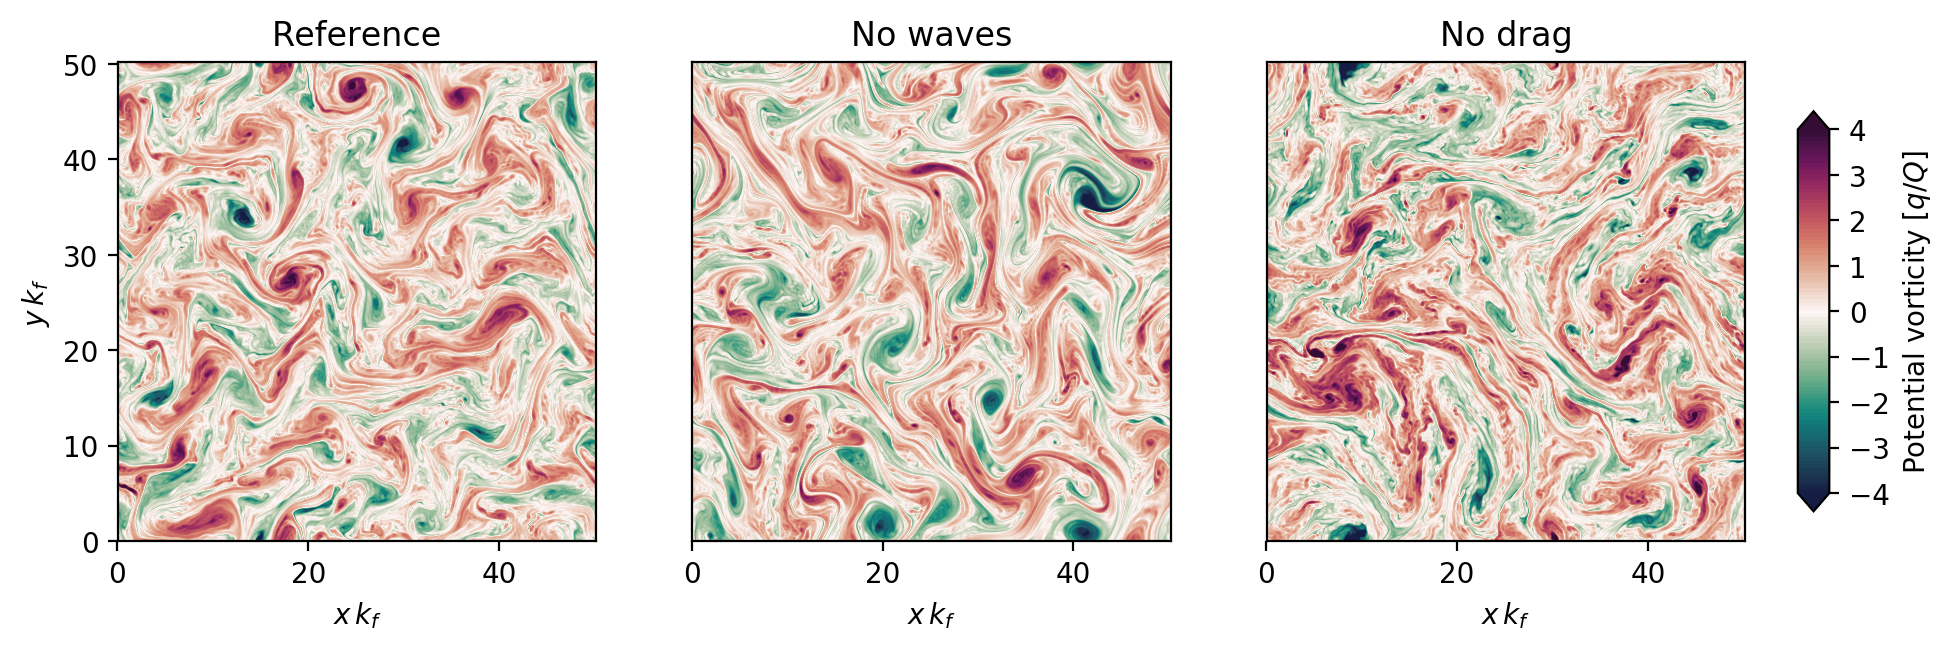
\includegraphics[width=1.\textwidth]{figs/snapshots_pv_t_60.png}
\caption{Snapshots of potential vorticity at $t\gamma  = 60$ of the three simulations.
          The normalization constant is $Q = k_f U_e$.}
        \label{equilibrated_pv}
\end{figure}

\begin{figure}
\centering
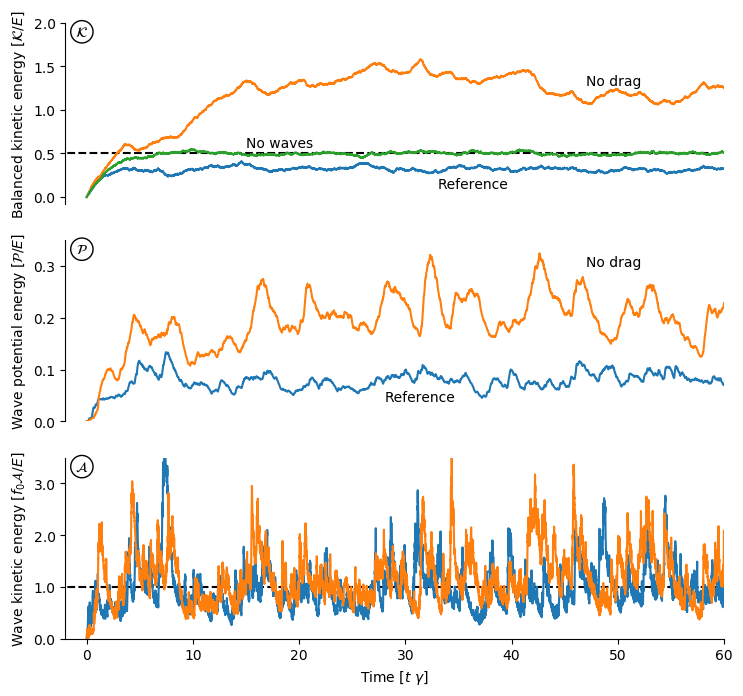
\includegraphics[width=.825\textwidth]{figs/energies_comparison.png}
\caption{Time series of balanced kinetic energy $\K$,   wave kinetic energy $f_0\A$,
          and wave potential energy $\P$ for the three simulations. The normalization
          constant is the predicted wave kinetic energy, $E = \sigma_w^2/2\gamma$.}
        \label{equilibrated_energy}
\end{figure}

\subsection{Energy budgets}
Figures \ref{energy_budgets_reference} and \ref{energy_budgets_nodrag} show the
energy budgets of the reference and non-wave solutions. Starting from the wave kinetic
energy budget, the power delivered by the random force is removed via linear dissipation.
While after equilibration the forcing work is nearly constant, the linear dissipation displays
large fluctuations, which explains the intermittency of $f_0\A$ in figure \ref{equilibrated_energy}.

\begin{figure}
\centering
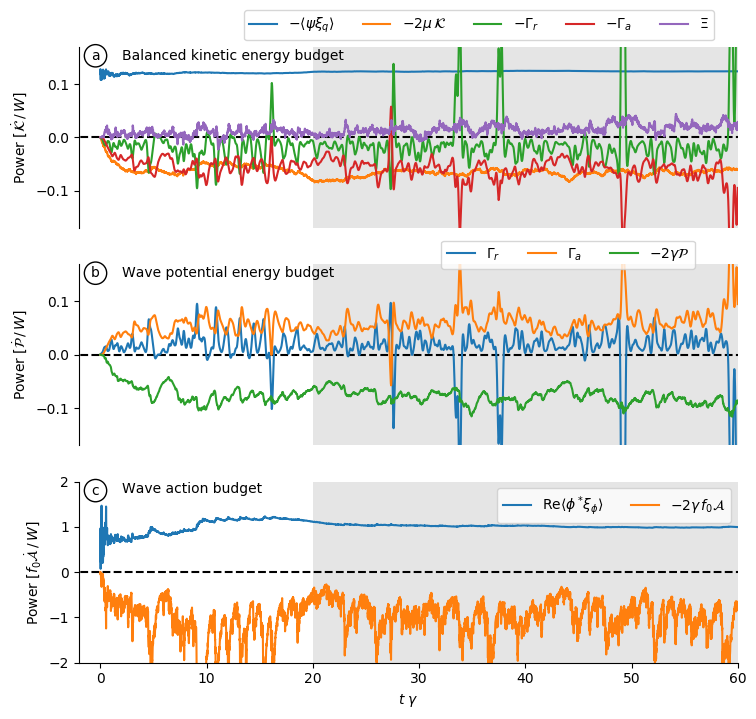
\includegraphics[width=.825\textwidth]{figs/K_and_P_and_A_budget_reference.png}
\caption{The budget of (a) balanced kinetic energy ($\K$), wave potential energy ($\P$),
        and (c) wave kinetic energy ($f_0 \A$)  for the solution with parameters in table
         \ref{parameters_reference}. The power is scaled by the work due to the
         wave forcing $W=\sigma_w^2/2$.}
        \label{energy_budgets_reference}
\end{figure}
\begin{figure}
\centering
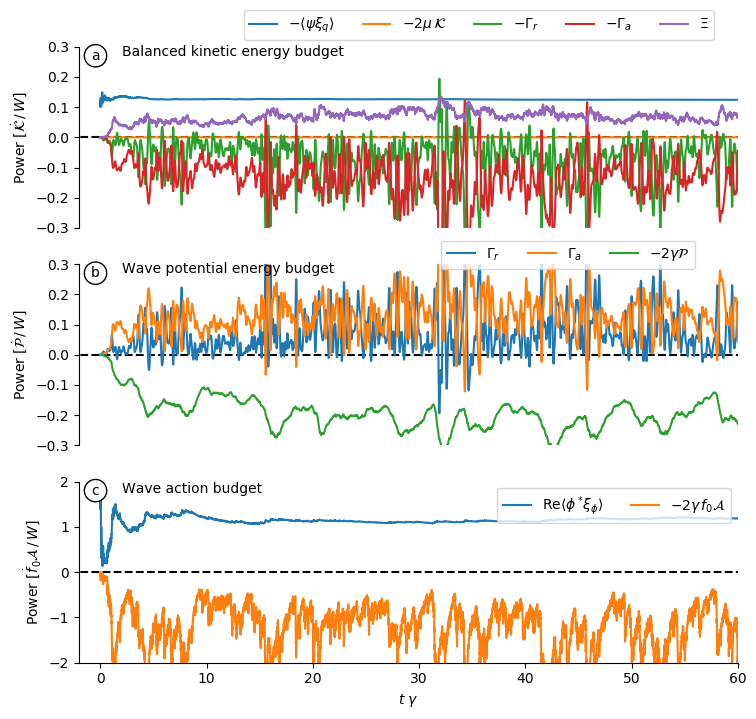
\includegraphics[width=.825\textwidth]{figs/K_and_P_and_A_budget_nodrag.png}
\caption{The budget of (a) balanced kinetic energy ($\K$), wave potential energy ($\P$),
        and (c) wave
         kinetic energy ($f_0 \A$)  for the solution with parameters in table
         \ref{parameters_reference}. The power is scaled by the work due to the
         wave forcing $W=\sigma_w^2/2$.}
        \label{energy_budgets_nodrag}
\end{figure}

\begin{table}
 \begin{center}
   \caption{Balanced kinetic energy budget of the reference and no-drag and no-wave solutions.
              Each term is normalized by the predicted amount of power delivered by
              the random force, $\sigma_q^2$.}
   \label{K-budgets}
   \begin{tabular}{ l | c | c | c }
     \hline
       &  Reference & No-drag & No-wave \\
      \hline
      Work & 1.00 &   1.00   &  1.00\\
      Streamming & 0.24 & 0.60 & --\\
      Stimulated generation & -0.64 & -1.77 & --\\
      Linear drag & -0.67 & -- & -0.99\\
      Residual. & -0.08 & 0.17 & -0.01\\
   \end{tabular}
\end{center}
\end{table}


\begin{table}
 \begin{center}
   \caption{Wave kinetic energy budget of the reference and no-drag solutions.
              Values represent averages after equilibration, normalized by the work
              delivered the random force, $\sigma_w^2/2$.}
   \label{A-budgets}
   \begin{tabular}{ l | c | c }
     \hline
       &  Reference & No-drag  \\
      \hline
      Work & 1.00 &   1.00   \\
      Linear diss. & -1.06 & --\\
      Residual & 0.04 & 0.06 \\
   \end{tabular}
 \end{center}
\end{table}

\begin{table}
 \begin{center}
   \caption{Wave potential energy budget of the reference and no-drag solutions.
              Values represent averages after equilibration, normalized by the production
              of wave potential energy via stimulated generation, $\Gamma_r + \Gamma_a$.}
   \label{P-budgets}
   \begin{tabular}{ l | c | c }
     \hline
       &  Reference & No-drag  \\
      \hline
      Refractive conversion & 0.32  & 0.37 \\
      Advective conversion  & 0.68  & 0.63 \\
      Linear dissipation & -0.99 & -0.97\\
      Residual & -0.01 & -0.03\\
   \end{tabular}
 \end{center}
\end{table}

%
% Bibliography
%

\clearpage
\bibliography{ForcedQGNIW.bib}


\end{document}
